\subsection{Mokymo klasė}
\label{subsec:trainer}

Klasė \texttt{Trainer} apibendrina visą modelio mokymo, validavimo ir testavimo gyvenimo ciklą: kviečia pirmyninį ir atgalinį žingsnius, kaupia metrikas, generuoja klasifikavimo matricą ir spėjimų pavyzdžius (žr.~\ref{fig:trainer_class_first} – \ref{fig:trainer_class_last} pav.).

\begin{figure}[H]
    \centering
    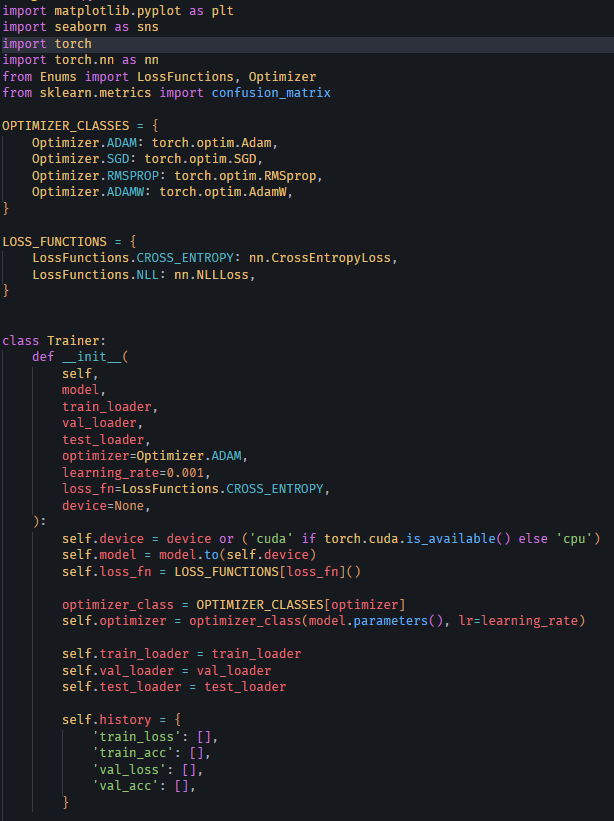
\includegraphics[width=0.85\linewidth]{3Lab/overleaf/images/Trainer_Class_1.png}
    \caption{Mokymo klasės kodas I dalis.}
    \label{fig:trainer_class_first}
\end{figure}

\begin{figure}[H]
    \centering
    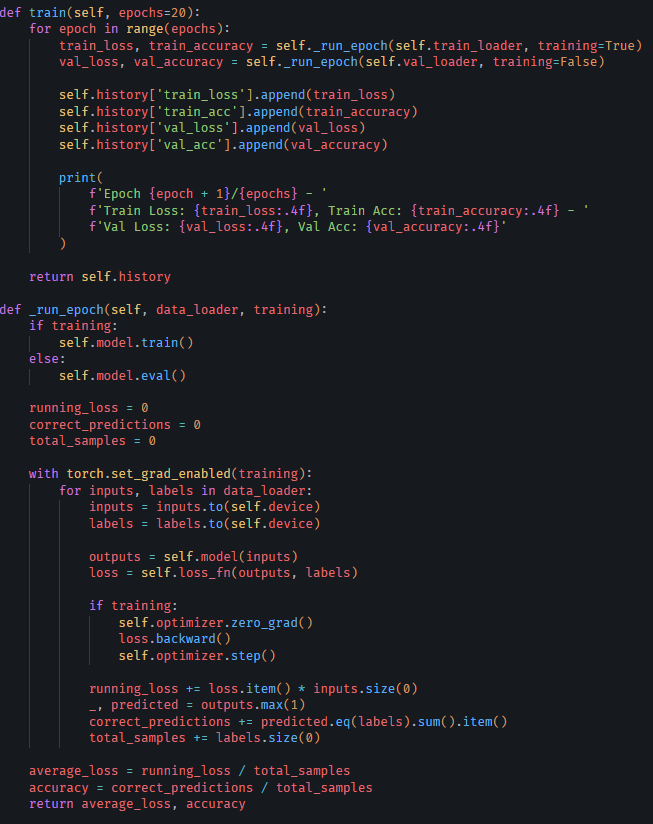
\includegraphics[width=0.85\linewidth]{3Lab/overleaf/images/Trainer_Class_2.png}
    \caption{Mokymo klasės kodas II dalis.}
    \label{fig:trainer_class_2}
\end{figure}

\begin{figure}[H]
    \centering
    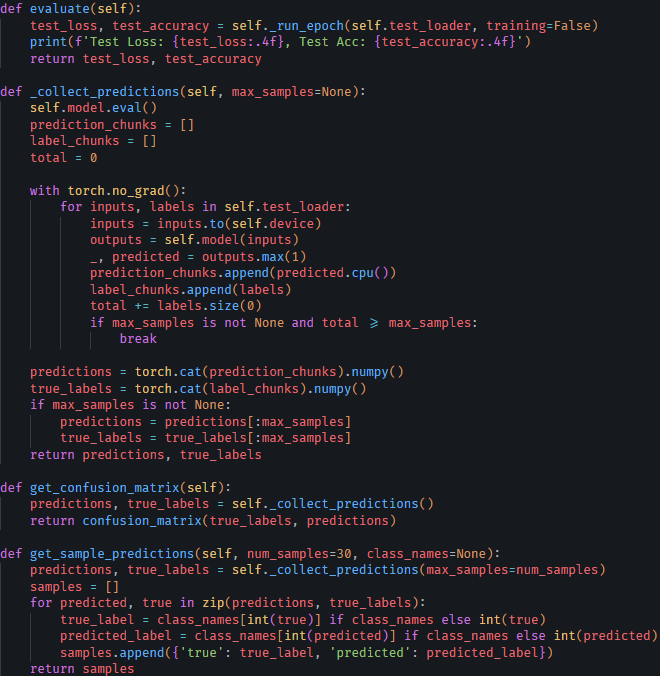
\includegraphics[width=0.85\linewidth]{3Lab/overleaf/images/Trainer_Class_3.png}
    \caption{Mokymo klasės kodas III dalis.}
    \label{fig:trainer_class_3}
\end{figure}

\begin{figure}[H]
    \centering
    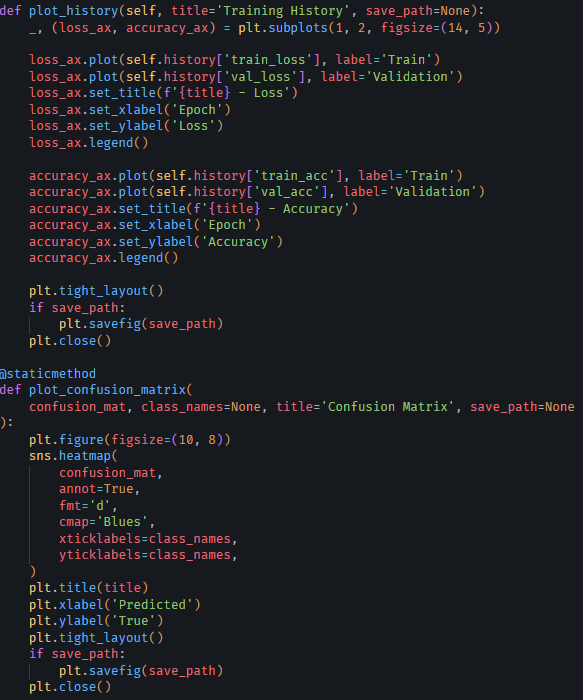
\includegraphics[width=0.85\linewidth]{3Lab/overleaf/images/Trainer_Class_4.png}
    \caption{Mokymo klasės kodas IV dalis.}
    \label{fig:trainer_class_4}
\end{figure}

\begin{figure}[H]
    \centering
    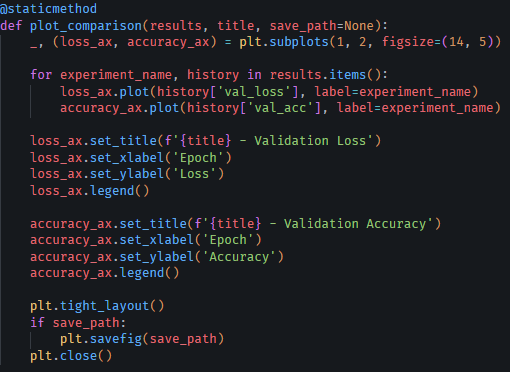
\includegraphics[width=0.85\linewidth]{3Lab/overleaf/images/Trainer_Class_5.png}
    \caption{Mokymo klasės kodas V dalis.}
    \label{fig:trainer_class_last}
\end{figure}

Klasės atsakomybės:
\begin{itemize}
    \item \texttt{train(epochs)} – kviečia \texttt{\_run\_epoch} mokymo ir validavimo aibėms kiekvienoje epochoje; kaupia keturių metrikų istoriją (\texttt{train\_loss}, \texttt{train\_acc}, \texttt{val\_loss}, \texttt{val\_acc}).
    \item \texttt{\_run\_epoch} – vienos epochos ciklas. Mokymo režime perjungia \texttt{model.train()}, validavimo / testavimo – \texttt{model.eval()}. Pagrindiniai žingsniai: paskaičiuoti \texttt{loss}, atlikti \texttt{loss.backward()} ir \texttt{optimizer.step()}, sumuoti tikslumą.
    \item \texttt{evaluate} – paleidžia tinklą ant testavimo aibės be gradiento skaičiavimo (\texttt{torch.no\_grad}).
    \item \texttt{get\_confusion\_matrix} – surenka spėjimus visam testavimo \texttt{DataLoader}'iui ir kviečia \texttt{sklearn.metrics.confusion\_matrix}.
    \item \texttt{get\_sample\_predictions(num\_samples)} – grąžina pirmųjų \texttt{num\_samples} testinių įrašų spėjimus su tikromis klasėmis (panaudota $30$ pavyzdžių sekcijoje).
    \item \texttt{plot\_history}, \texttt{plot\_confusion\_matrix}, \texttt{plot\_comparison} – \texttt{matplotlib} ir \texttt{seaborn} grafikai eksperimentų vizualizavimui.
\end{itemize}

Mokymo metu naudojamas:
\begin{itemize}
    \item \textbf{Paklaidos funkcija} \texttt{nn.CrossEntropyLoss} – matuoja, kaip toli tinklo \textit{logits} nuo tikrų klasių (žemo tikslumo prognozės baudžiamos labiau).
    \item \textbf{Optimizatorius} – konfigūruojamas per \texttt{Optimizer} enumeraciją (\textit{Adam} pagal nutylėjimą).
    \item \textbf{Tikslumo skaičiavimas} – \texttt{outputs.max(1)} grąžina kiekvienai eilutei didžiausios \textit{logit} reikšmės indeksą; lyginama su tikra klase.
\end{itemize}

Klasės architektūra ir mokymo ciklas suprogramuoti autoriaus. \texttt{matplotlib} / \texttt{seaborn} grafikų braižymo metodų \texttt{plot\_history}, \texttt{plot\_confusion\_matrix} ir \texttt{plot\_comparison} kvietimo šablonams panaudotos Claude pasiūlytos paruoštos formos, kurios vėliau pritaikytos prie projekto poreikių.
